\chapter{The NoBeard Machine Architecture}
\section{The NoBeard Machine}
It is a virtual machine with an instruction set of 31 instructions which is pretty easy to understand compared to the instruction set sizes of real life machines. The machine is purely stack based such that the structure of each instruction is easy to grasp and to follow. The machine has a word width of four bytes and is being target for NoBeard programs. The NoBeard Machine consists of the following components.
\begin{figure}[h] 
	\centering
	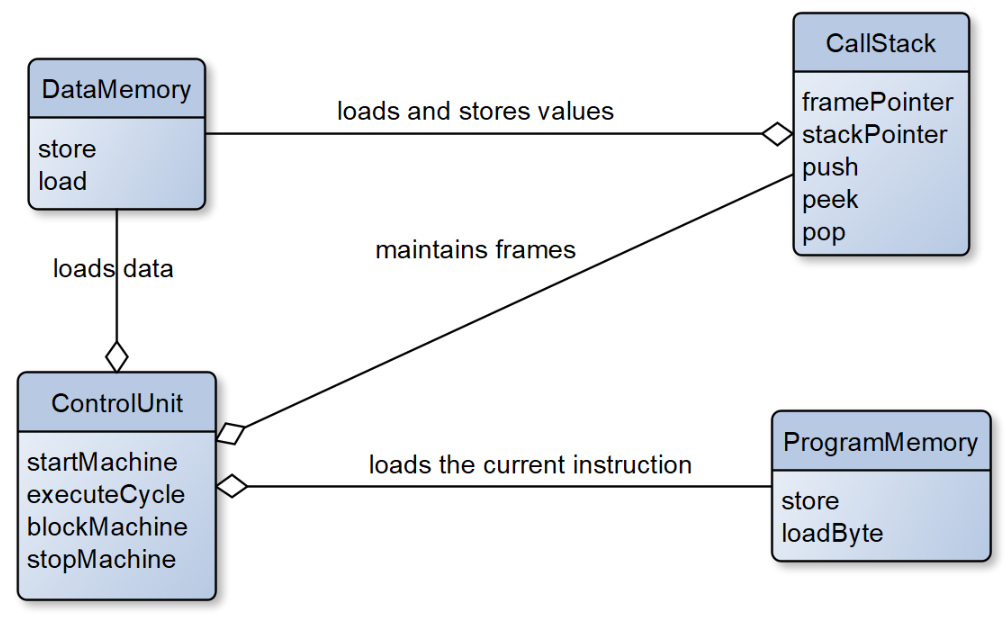
\includegraphics[scale=.62]{images/componentsOfNbM.png}
	\caption{Components of the NoBeardMachine Architecture}
	\label{fig:componentsOfNbM}
\end{figure}
\subsection{Program Memory}
The program memory stores instructions with belonging opcode and operands. It is byte addressed memory with a specified maximum size. Addresses access outside the range of 0 to the maximum size -1 lead to a “ProgramAddressError”.
\subsection{Data Memory} 
\label{ssec:dataMemory}
The Data memory is a storage which is byte addressed and stores variables in the following way:
\begin{itemize}
\item \textbf{Characters }are one-byte values are stored byte wise into the data memory. 
\item \textbf{Integers }are four-byte values and are stored in little endian order. Negative integer values are stored as Two’s Complement (see \cite{wikipedia_twos_2018}).
\item \textbf{Booleans }are four-bytes values and are stored as the integer 0 for false and the integer 1 for true.
\end{itemize}

\begin{figure}[h]
\begin{center}
\begin{tabular}{p{8em}|p{8em}|}
\cline{2-2}
\parbox[t][3em][t]{8em}{\hfill 0} & String Constants \\[3em] \cline{2-2}
& Stack frame 1 \\[2em] \cline{2-2}
& Stack frame 2 \\[2em] \cline{2-2}
& \ldots \\[2em] \cline{2-2}
\parbox[b][4em][b]{8em}{\hfill MAX\_DATA} & free \\ \cline{2-2}
\end{tabular}
\end{center}
\caption{Data Memory of the NoBeard Machine}\label{fig:datamemory}
\end{figure}

As figure~\ref{fig:datamemory} shows, the data memory is separated into two parts, string constants and to stack frames of the currently running functions. 
\subsubsection{String Constants}
String constants in NoBeard assembler programs are written at the beginning of the source code under quotation marks. It includes all strings that has to be printed out on the console. Before starting a program on the virtual machine string constants are stored in the constant memory. 
\subsubsection{Stack Frames}
After the constant memory the stack frames are maintained in a certain way. For every execution of a function a new frame is added. It holds data for the functions arguments, local variables and its expression stack. As soon as functions ends, its frame is removed. 

\begin{figure}[h]
\begin{center}
\begin{tabular}{p{8em}|p{4em}|p{15em}}
\parbox[b][1em][b]{8em}{\hfill \cellcolor{Gray}\textcolor{White}{Address}} & \cellcolor{Gray}\textcolor{White}{Content} & \cellcolor{Gray}\textcolor{White}{Remark} \\ \cline{2-2} 
\cline{2-2}
\parbox[t][1em][t]{5em}{\hfill 0} & 0 & frame pointer of frame 0 \\ \cline{2-2}
& \ldots \\ \cline{2-2}
\parbox[t][1em][t]{5em}{\hfill 32} & 13 & local int in frame 0 \\ \cline{2-2}
\parbox[t][1em][t]{5em}{\hfill 36} & 0 & static link to frame 0 (start of frame 1)\\ \cline{2-2}
& \ldots \\ \cline{2-2}
\parbox[t][1em][t]{5em}{\hfill 68} & 17 & local int in frame 1\\ \cline{2-2}
\parbox[t][1em][t]{5em}{\hfill 72} & 42 & local int in frame 1\\ \cline{2-2}
\parbox[t][1em][t]{5em}{\hfill 76} & 36 & static link to frame 1 (start of frame 2) \\ \cline{2-2}
& \ldots \\ \cline{2-2}
\parbox[t][1em][t]{5em}{\hfill 108} & `D' \\ \cline{2-2}
\parbox[t][1em][t]{5em}{\hfill 109} & 61 \\ \cline{2-2}
\parbox[b][4em][b]{8em}{\hfill MAX\_DATA} & free \\ \cline{2-2}
\end{tabular}
\end{center}
\caption{Snapshot of a call stack with three frames}\label{fig:threeframes}
\end{figure}

Figure~\ref{fig:threeframes} shows a pretty good example from \cite{bauer_p._2017}. Here we can see that the memory is working with three frames. Frame~0 starts at address 0. The first 32 bytes of each frame are reserved for administrative data like the static link and the dynamic link to the surrounding frame, the return value, etc. Address~32 holds the value of a local variable in frame~0.

\lstset{language=NoBeardAsm}

At address~36 frame~1 starts with the address to its statically surrounding frame, i.e, the function (or unit or block) represented by frame~0 is defining the function (or block) represented by frame~1. Frame~1 defines two local values at addresses 68 and 72. Now it can be easily verified that an assembler instruction \lstinline$la 0 32$ (see section~\ref{sec:instructions}) loads the value of the local (i.e., relative to the closest frame pointer) address 32. In the concrete example this is address $36 + 32 = 68$.

\subsection{Call Stack}
By structuring the data memory as a stack the call stack is needed as an abstraction to the data memory. With the help of different functions the call stack is able to add and remove frames from the stack and to maintain the expression stack. Data that are needed for each statement get stored in the expression stack. It grows and shrinks as needed and is empty at the end of each statement. The stack is addressed word-wise only. The call stack has the two major components:

\begin{itemize}
\item \textbf{Stack Pointer: }Address of the start of the last used word on the stack. 
\item \textbf{Frame Pointer: }Address of the first byte of the currently running function's stack frame. 
\end{itemize}

\subsection{Control Unit}
It is responsible for the program work flow. It executes one machine cycle in three steps, it fetches, decodes and operates the current instruction. Depending on some instruction, the control unit also affect the state of the machine. To achieve these steps it has to work with the following components:

\begin{itemize}
\item \textbf{Program Counter: }Start address of the next instruction to be executed.
\item \textbf{Machine State: }The NoBeard machine has four different states and is always in one of them. 
	\begin{itemize}
		\item \lstinline$running$: The machine runs
		\item \lstinline$stopped$: The machine stops. Usually when the end of program is reached.
		\item \lstinline$blocked$: The machine pauses. Mostly when a breakpoint is placed by the user.
		\item \lstinline$error$: Error state
	\end{itemize}
\end{itemize}

\section{Binary File Format}
The virtual machine runs only NoBeard object files with extension \lstinline$.no$ which can be generated by an NoBeard Assembler or NoBeard Compiler. From the first byte onwards the machine instructions are stored in a continuous flow. After a final \lstinline$halt$ instruction the stream of string constants is stored. This is also shown in figure~\ref{fig:binaryfileformat}.

\begin{figure}[h]
\begin{center}
\begin{tabular}{p{8em}|p{8em}|}
\cline{2-2}
\parbox[t][3em][t]{8em}{\hfill 0} & Instructions \\[3em] \cline{2-2}
\parbox[b][2em][b]{8em}{\hfill N} & String Constants \\ \cline{2-2}
\end{tabular}
\end{center}
\caption{NoBeard Binary File Format}\label{fig:binaryfileformat}
\end{figure}

\section{Runtime Structure of NoBeard Program}
The machine has a firmly defined execution cycle:
\begin{enumerate}
\item Fetch instruction
\item Decode instruction
\item Execute instruction
\end{enumerate}
The very first instruction is fetched from a specified starting program counter which is provided as an argument when starting the program. From this point of time forwards the program is running until the machine state changes from run. There are two options to interrupt the machine from running state. It get interrupted mostly by the debugger with a breakpoint. Or otherwise when the \lstinline$halt$ instruction get executed.
\section{Instructions}\label{sec:instructions}
NoBeard instructions are of a different length and each has an opcode and operands of an amount between 0 and 2. The first byte of all instructions is reserved for the op code, which is the identifier used to identify the instruction on machine language level. The remaining bytes, if any, are assigned to the operand of the instruction.
Each of the following subsections explains these instructions in four categories. The underlined title is the shorthand that identifies the instruction on assembler level. Then follows a table showing the size of the instruction and which bytes carry which information. Finally, each one has also a short explanation in human language and in some cases also an example. All the examples here are taken from \cite{bauer_p._2017}.

\subsection{Load and Store Instructions}
% ----------------------------- NOP ----------------------------
\subsubsection{nop}
\onebyteinstruction{0x00}

\paragraph{Operation:}
Empty instruction. Does nothing

\begin{lstlisting}
nop
\end{lstlisting}

% ----------------------------- LIT ----------------------------
\subsubsection{lit}
\threebyteinstruction{0x01}{Literal}

\paragraph{Operation:}
Pushes a value on the expression stack.

\begin{lstlisting}
lit Literal
push(Literal);
\end{lstlisting}


% ----------------------------- LA ----------------------------
\subsubsection{la}
\fourbyteinstructiona{0x02}{Displacement}{DataAddress}

\paragraph{Operation:}
Loads an address on the stack.

	\begin{lstlisting}
	la Displacement DataAddress
	base = fp;
	for (i= 0; i < Displacement; i++) {
		base = dat[base ... base + 3];
	}
	push(base + DataAddress);
	\end{lstlisting}

% ----------------------------- LV ----------------------------
\subsubsection{lv}
\fourbyteinstructiona{0x03}{Displacement}{DataAddress}

\paragraph{Operation:}
Loads a value on the stack.

	\begin{lstlisting}
	lv Displacement DataAddress
	base = fp;
	for (i = 0; i < Displacement; i++) {
		base = dat[base ... base + 3];
	}
	adr = base + DataAddress;
	push(dat[addr ... addr + 3]);
	\end{lstlisting}

% ----------------------------- LC ----------------------------
\subsubsection{lc}
\fourbyteinstructiona{0x04}{Displacement}{DataAddress}

\paragraph{Operation:}
Loads a character on the stack.

	\begin{lstlisting}
	lc Displacement DataAddress
	base = fp;
	for (i = 0; i < Displacement; i++) {
		base = dat[base ... base + 3];
	}
	// fill 3 bytes of zeros to get a full word
	lw = 000dat[base + Address];
	push(lw);
	\end{lstlisting}

% ----------------------------- LVI ----------------------------
\subsubsection{lvi}
\fourbyteinstructiona{0x03}{Displacement}{DataAddress}

\paragraph{Operation:}
Loads a value indirectly on the stack.

	\begin{lstlisting}
	lvi Displacement DataAddress
	base = fp;
	for (i = 0; i < Displacement; i++) {
		base = dat[base ... base + 3];
	}
	adr = base + DataAddress;
	ra = dat[addr ... addr + 3];
	push(ra);
	\end{lstlisting}

% ----------------------------- LCI ----------------------------
\subsubsection{lci}
\fourbyteinstructiona{0x05}{Displacement}{DataAddress}

\paragraph{Operation:}
Loads a character indirectly on the stack.

	\begin{lstlisting}
	lci Displacement DataAddress
	base = fp;
	for (i = 0; i < Displacement; i++) {
		base = dat[base ... base + 3];
	}
	ra = dat[base + Address];
	// fill 3 bytes of zeros to get a full word
	lw = 000dat[ra];
	push(lw);
	\end{lstlisting}

% ----------------------------- INC ----------------------------
\subsubsection{inc}
\threebyteinstruction{0x1D}{Size}

\paragraph{Operation:}
Increases the size of the stack frame by \lstinline$Size$.

	\begin{lstlisting}
	inc Size
	top += Size;
	\end{lstlisting}

% ----------------------------- STO ----------------------------
\subsubsection{sto}
\onebyteinstruction{0x07}

\paragraph{Operation:}
Stores a value on an address.

	\begin{lstlisting}
	sto
	x = pop();
	a = pop();
	dat[a ... a + 3] = x;
	\end{lstlisting}

% ----------------------------- STC ----------------------------
\subsubsection{stc}
\onebyteinstruction{0x08}

\paragraph{Operation:}
Stores a character on an address.

	\begin{lstlisting}
	stc
	x = pop();
	a = pop();
	// Only take the rightmost byte
	dat[a] = 000x;
	\end{lstlisting}

\subsection{Integer Instructions}


% ----------------------------- NEG ----------------------------
\subsubsection{neg}
\onebyteinstruction{0x0B}

\paragraph{Operation:}
Negates the top of the stack.

	\begin{lstlisting}
	neg
	x = pop();
	push(-x);
	\end{lstlisting}

% ----------------------------- ADD ----------------------------
\subsubsection{add}
\onebyteinstruction{0x0C}

\paragraph{Operation:}
Adds the top two values of the stack.

	\begin{lstlisting}
	add
	push(pop() + pop());
	\end{lstlisting}

% ----------------------------- SUB ----------------------------
\subsubsection{sub}
\onebyteinstruction{0x0D}

\paragraph{Operation:}
Subtracts the top two values of the stack.

	\begin{lstlisting}
	sub
	y = pop();
	x = pop();
	push(x - y);
	\end{lstlisting}

% ----------------------------- MUL ----------------------------
\subsubsection{mul}
\onebyteinstruction{0x0E}

\paragraph{Operation:}
Multiplies the top two values of the stack.

	\begin{lstlisting}
	mul
	push(pop() * pop());
	\end{lstlisting}

% ----------------------------- DIV ----------------------------
\subsubsection{div}
\onebyteinstruction{0x0F}

\paragraph{Operation:}
Divides the top two values of the stack.

	\begin{lstlisting}
	div
	y = pop();
	x = pop();
	if (y != 0)
		push(x / y);
	else
		throwDivByZero();
	\end{lstlisting}


% ----------------------------- MOD ----------------------------
\subsubsection{mod}
\onebyteinstruction{0x10}

\paragraph{Operation:}
Calculates the remainder of the division of the top values of the stack.

	\begin{lstlisting}
	mod
	y = pop();
	x = pop();
	push(x % y);
	\end{lstlisting}

% ----------------------------- NOT ----------------------------
\subsubsection{not}
\onebyteinstruction{0x11}

\paragraph{Operation:}
Calculates the remainder of the division of the top values of the stack.

	\begin{lstlisting}
	not
	x = pop();
	if (x == 0)
	   push(1);
	else
	   push(0);
	\end{lstlisting}

\subsection{Control Flow Instructions}

% ----------------------------- FJMP ----------------------------
\subsubsection{fjmp}
\threebyteinstruction{0x16}{NewPc}

\paragraph{Operation:}
Sets \lstinline$pc$ to \lstinline$newPc$ if stack top value is false.

	\begin{lstlisting}
	fjmp newPc
	x = pop();
	if (x == 0)
	   pc = NewPc;
	\end{lstlisting}

% ----------------------------- TJMP ----------------------------
\subsubsection{tjmp}
\threebyteinstruction{0x17}{NewPc}

\paragraph{Operation:}
Sets \lstinline$pc$ to \lstinline$newPc$ if stack top value is true.

	\begin{lstlisting}
	tjmp newPc
	x = pop();
	if (x == 1)
	   pc = NewPc;
	\end{lstlisting}

% ----------------------------- JMP ----------------------------
\subsubsection{jmp}
\threebyteinstruction{0x18}{NewPc}

\paragraph{Operation:}
Unconditional jump: Sets \lstinline$pc$ to \lstinline$newPc$.

	\begin{lstlisting}
	jmp newPc
	pc = NewPc;
	\end{lstlisting}

% ----------------------------- BREAK----------------------------
\subsubsection{break}
\onebyteinstruction{0x1F}

\paragraph{Operation:}
Breaks the machine. Especially used for the debugging function.

	\begin{lstlisting}
	break
	ms = blocked;
	\end{lstlisting}

% ----------------------------- HALT ----------------------------
\subsubsection{halt}
\onebyteinstruction{0x1F}

\paragraph{Operation:}
Halts the machine.

	\begin{lstlisting}
	halt
	ms = stopped;
	\end{lstlisting}
	

\subsection{IO-Instructions}

% ----------------------------- IN ----------------------------
\subsubsection{in}\label{sec:in}
\twobyteinstruction{0x19}{Type}

\paragraph{Operation:}
Reads data from the terminal. Depending on \lstinline$Type$ different data types are read:

\begin{itemize}
	\item 0: An \lstinline$int$ is read and stored at the address on top of the stack. After execution the value 1 is pushed if an integer was read successfully, otherwise 0 is pushed.
	\item 1: A \lstinline$char$ is read and stored at the address on top of the stack. After execution the value 1 is pushed 
	\item 2: a \lstinline$string$ with a specific length is read
\end{itemize}

	\begin{lstlisting}
	in Type
	switch(Type) {
		case 0:
			a = pop();
			n = readInt();
			dat[a ... a + 3] = n;
			break;
		case 1:
			a= pop();
			ch = readChar();
			dat[a] = ch;
			break;
		case 2:
			a = pop();
			strLen = pop();
			
			break;
	}
	\end{lstlisting}

% ----------------------------- OUT ----------------------------
\subsubsection{out}\label{sec:out}
\twobyteinstruction{0x1A}{Type}

\paragraph{Operation:}
Writes data to the terminal. Depending on \lstinline$Type$ different data types are printed:

\begin{itemize}
	\item 0: An \lstinline$int$ with a specific column width is printed
	\item 1: A \lstinline$char$ with a specific column width is printed
	\item 2: a \lstinline$string$ with a specific column width is printed
	\item 3: a new line is printed
\end{itemize}

	\begin{lstlisting}
	out Type
	switch(Type) {
		case 0:
			width = pop();
			x = pop();
			// + means string concatenation in the next line
			formatString = "%" + width + "d";
			printf(formatString, x);
			break;
		case 1:
			width= pop();
			x = pop();
			printf("%c", x);
			for (i = 0; i < width - 1; i++)
				printf(" ");
			break;
		case 2:
			width = pop();
			strLen = pop();
			strAddr = pop();
			printf("%s", dat[strAddr ... strAddr + strLen - 1]);
			for (i = n; i < width - 1; i++)
				printf(" ");
			break;
		case 3:
			printf("\n");
			break;
	}
	\end{lstlisting}
	
\section{NoBeard Assembler}
To write programs for the NoBeard machine an Assembler is provided. NoBeard Assembler files are separated in two blocks, which is called the string constants and the assembler program. The files have the extensions \lstinline$.na$ for NoBeard Assembler. The string constants are stored between two double quotes and has to be located at the beginning of the file. There is no way to address a single constant. So, if we use a string constant in the assembler program, we have to specify the starting address of the string constant and the length needed in the program. Assembler programs  contain a sequence of assembler instructions like \lstinline$lit$ for load or \lstinline$out$ for print. After the opcode of the instruction follows the operands, if they are needed as already described in section \ref{sec:instructions}.
\subsection{Example}
